
\chapter{Theoretical background}%
\label{ch:theory}

\section{Ultrasound}
\label{sec:theory_ultrasound}

Ultrasound is defined as sound waves with frequencies above the upper limit of human hearing, which is typically around 20 kHz. 

\subsection{Transducer}

\subsection{Reflection and Scattering}

\subsection{Attenuation}

\subsection{Time of Flight}

\subsection{Noise sources}

\section{Pulsed-Wave Doppler}
\label{sec:theory_pw_doppler}

In the present system, \gls{PW Doppler} is used to measure the blood flow velocity. It works by emitting a series of high frequency sound pulses into the tissue at a constant \gls{PRF}. Each pulse consists of a burst of sound waves with a pulse center frequency $f_c$ with $N_{cycles}$ cycles. The pulse length $T$ is then given by $T = N_{cycles} / f_c$. After a pulse is emitted, the system records the returning echoes. This is commonly referred to as the \textit{fast time} signal. The fast time signal is sampled with a sampling rate $f_{s, FT}$

\begin{table}[h]
    \centering
    \begin{tabular}{ccc}
        \hline
        Parameter & Symbol & Value \\
        \hline
        Pulse center frequency & $f_c$ & \SI{8}{\mega\hertz}\\
        Number of cycles & $N_{cycles}$ & 12 \\
        Pulse length & $T$ & \SI{1.5}{\micro\second} \\
        Pulse repetition frequency & \gls{PRF} & \SI{20}{\kilo\hertz} \\
        Speed of sound in tissue & $c$ & \SI{1540}{\meter\per\second} \\
        \hline
    \end{tabular}
\end{table}

\begin{figure}
    \centering
    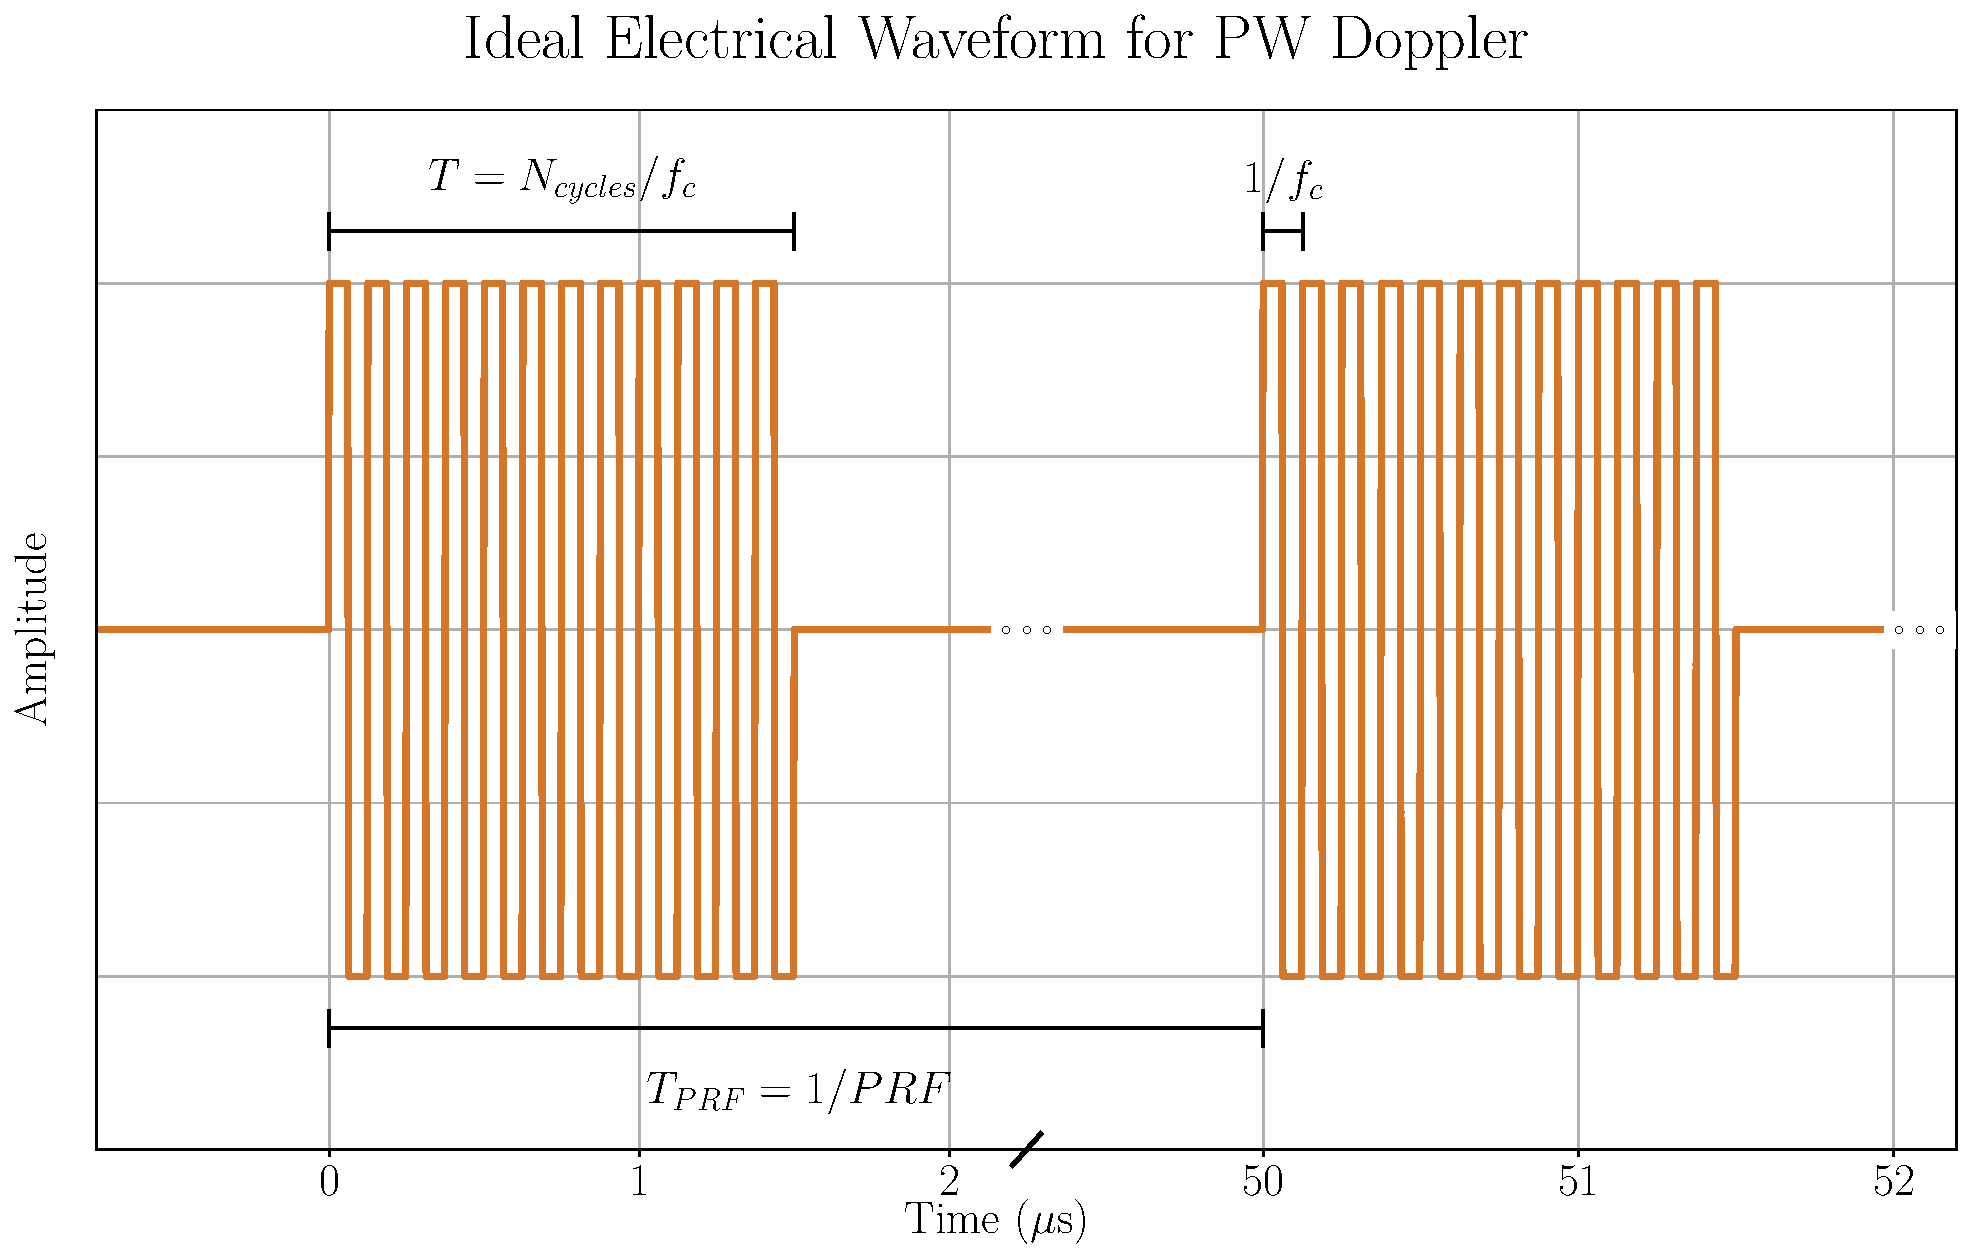
\includegraphics[width=1.0\textwidth]{../../code/figures/theory/emitted_waveform.pdf}
    \caption{Ideal emitted electrical waveform for \gls{PW Doppler}, with annotations. Note that the time axis is broken to show the pulse repetition period.}
    \label{fig:theory_ideal_emitted_wave}
\end{figure}

\subsection{Decimation}

\subsection{Clutter Filter}